\section{The bias-variance relationship}\label{sec:bv}

Understanding over and under-fitting is very important to understanding the challenges faced when doing machine learning. As it turns out those concepts are fundamentally tied to the out-of-sample error, $E_{out}$, for which the least squares cost function can be decomposed in three contributions\footnote{This is shown by \citet{Mehta2019} and we refer to that work for details on the derivation}, namely

\begin{align}\label{eq:bv_decomp}
E_{out} = \langle C(\mathbf{\hat{y}}^t, f(\mathbf{x}^t; \theta^*_S))\rangle_{S,\, \epsilon} = \text{Bias}^2 + \text{Variance} + \text{Noise}.
\end{align}

\noindent This expectation is rather compact and so before we move on to explaining the bias and variance start by elaborating on $S$ and $\epsilon$. Recall from equation \ref{eq:target} that we decompose the target values as a contribution from a true process and an error term $\epsilon$. The expectation over the cost then has a contribution from the noise, represented by the last term of the decomposition. Furthermore the expectation in equation \ref{eq:bv_decomp} is taken over a model with optimized parameters $\theta^*$, but that optimization can be thought to be a function of the selected data used in the optimization. We can then view $f(\mathbf{x}; \theta^*_S)$ as a stochastic functional which varies over the selected data $s = \{\mathbf{\hat{y}}, \mathbf{x}\}$ used for training. The expectation over $S$ is then an expectation over the set of different choices of training data, i.e. $S = \{s_i, s_{i+1}, \dots\}$. We also use the superscript $t$ on the outcome and state variables to indicate that they are from the testing set, variables without that subscript are implied to be from the training set.
 Using the derived quantities from \citet{Mehta2019}, and the notation described in the previous section and equation \ref{eq:target}, we can then define the bias as\todo{add some details on derivation?}

\begin{equation}\label{eq:bias}
\text{Bias}^2 := \sum_i (\mathbf{\hat{y}}_i^t - \langle f(\mathbf{x}_i^t; \theta_S^*)\rangle_S)^2.
\end{equation}

\noindent The bias term is analogous to the squared error cost and gives and estimate to the degree of under-fitting the model is susceptible to. Building on this we have the variance term, again using notation from this section, 

\begin{equation}\label{eq:variance}
\text{Variance} := \sum_i \langle (f(\mathbf{x}_i; \theta^*_S) - \langle f(\mathbf{x}_i; \theta^*_S) \rangle_S)\rangle_S.
\end{equation}

\noindent For clarity we note that the summation is over the testing set elements. The variance term relates to the consistency in the testing region, and as such describes the degree of over-fitting the model is exhibiting. Over-fitting is then a behavior intrinsically tied to the amount of data we have to train on (\cite{Mehta2019}). 

\begin{figure}
\centering
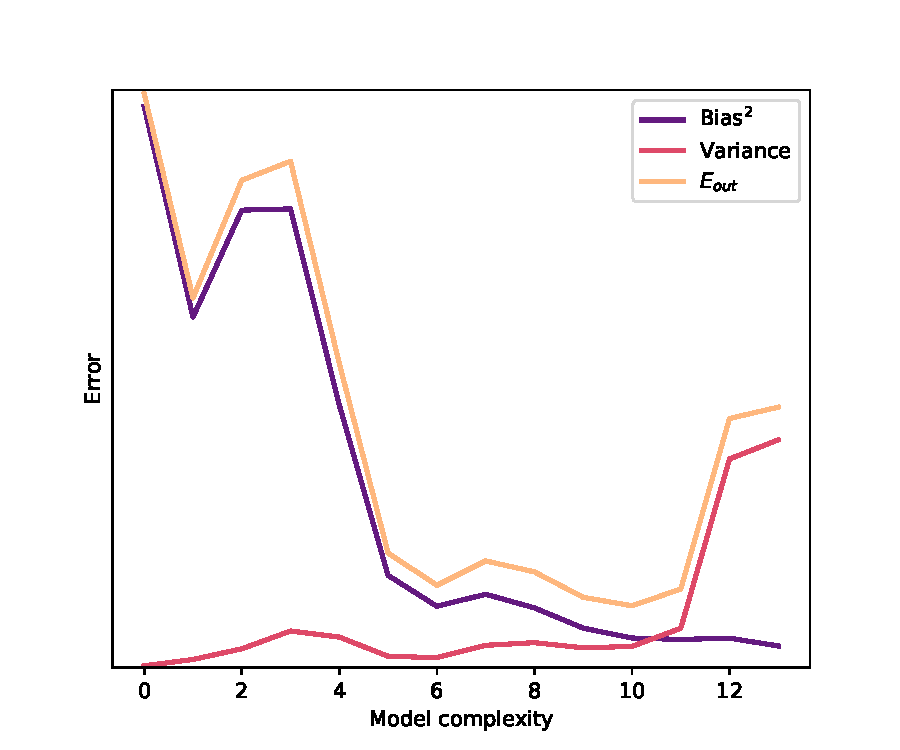
\includegraphics[width=0.55\textwidth, height=6.5cm]{../figures/bias_var_degree.pdf}
\caption[Bias-variance decomposition ]{Decomposition of the bias and variance from the overall test-set error $E_{out}$. A set of polynomials of varying degrees are fit to a known function using randomly selected training samples. The polynomial degree is denoted by the x-axis label. With the set of polynomials we evaluate the bias and variance terms shown in equation \ref{eq:bias} and \ref{eq:variance}. In the figure we observe the characteristic relationship where the out of sample error decreases steadily with complexity until the models start to over-fit as measured by the variance, and the $E_{out}$ increases as a consequence.}\label{fig:bv}
\end{figure}

The bias-variance relationship describes a fundamental challenge in most domains of machine learning; fitting a more complex model requires more data. Which has led to an explosion in the acquisition of vast amounts of data in the private sector. With the recent development in nuclear physics where data is becoming abundant this opens the avenue to exploring more complex models than has previously been possible. We illustrate this tension in figure \ref{fig:bv} where polynomials of varying degrees are fit to a linear combination of exponential functions. We observe the characteristic relationship between bias and variance wherein the out of sample error $E_{out}$ starts out decreasing with complexity, but increases exponentially as a threshold is reached. Note also that we illustrate the concept of the irreducible error that for a model class, i.e. polynomials, there is an irreducible error term owing to the contribution from the noise. 
